\documentclass[landscape,final,archE1,fontscale=0.3]{baposter}

\usepackage{calc}
\usepackage{graphicx}
\usepackage{amsmath}
\usepackage{amssymb}
\usepackage{relsize}
\usepackage{rotating}
\usepackage{bm}
\usepackage{url}
\usepackage{setspace}

\usepackage{tabularx}
\usepackage{graphicx}

\usepackage{palatino}
\usepackage{booktabs, multicol, multirow}

\usepackage[margin=1em]{caption}
\bibliographystyle{plain}

\graphicspath{{images/}{../images/}}
\usetikzlibrary{calc}

\newcommand{\SET}[1]  {\ensuremath{\mathcal{#1}}}
\newcommand{\MAT}[1]  {\ensuremath{\boldsymbol{#1}}}
\newcommand{\VEC}[1]  {\ensuremath{\boldsymbol{#1}}}
\newcommand{\Video}{\SET{V}}
\newcommand{\video}{\VEC{f}}
\newcommand{\track}{x}
\newcommand{\Track}{\SET T}
\newcommand{\LMs}{\SET L}
\newcommand{\lm}{l}
\newcommand{\PosE}{\SET P}
\newcommand{\posE}{\VEC p}
\newcommand{\negE}{\VEC n}
\newcommand{\NegE}{\SET N}
\newcommand{\Occluded}{\SET O}
\newcommand{\occluded}{o}

%%%%%%%%%%%%%%%%%%%%%%%%%%%%%%%%%%%%%%%%%%%%%%%%%%%%%%%%%%%%%%%%%%%%%%%%%%%%%%%%
%%%% Some math symbols used in the text
%%%%%%%%%%%%%%%%%%%%%%%%%%%%%%%%%%%%%%%%%%%%%%%%%%%%%%%%%%%%%%%%%%%%%%%%%%%%%%%%

%%%%%%%%%%%%%%%%%%%%%%%%%%%%%%%%%%%%%%%%%%%%%%%%%%%%%%%%%%%%%%%%%%%%%%%%%%%%%%%%
% Multicol Settings
%%%%%%%%%%%%%%%%%%%%%%%%%%%%%%%%%%%%%%%%%%%%%%%%%%%%%%%%%%%%%%%%%%%%%%%%%%%%%%%%
\setlength{\columnsep}{1.5em}
\setlength{\columnseprule}{0mm}

%%%%%%%%%%%%%%%%%%%%%%%%%%%%%%%%%%%%%%%%%%%%%%%%%%%%%%%%%%%%%%%%%%%%%%%%%%%%%%%%
% Save space in lists. Use this after the opening of the list
%%%%%%%%%%%%%%%%%%%%%%%%%%%%%%%%%%%%%%%%%%%%%%%%%%%%%%%%%%%%%%%%%%%%%%%%%%%%%%%%
\newcommand{\compresslist}{%
\setlength{\itemsep}{1pt}%
\setlength{\parskip}{0pt}%
\setlength{\parsep}{0pt}%
}

%%%%%%%%%%%%%%%%%%%%%%%%%%%%%%%%%%%%%%%%%%%%%%%%%%%%%%%%%%%%%%%%%%%%%%%%%%%%%%
%%% Begin of Document
%%%%%%%%%%%%%%%%%%%%%%%%%%%%%%%%%%%%%%%%%%%%%%%%%%%%%%%%%%%%%%%%%%%%%%%%%%%%%%

\begin{document}

%%%%%%%%%%%%%%%%%%%%%%%%%%%%%%%%%%%%%%%%%%%%%%%%%%%%%%%%%%%%%%%%%%%%%%%%%%%%%%
%%% Here starts the poster
%%%---------------------------------------------------------------------------
%%% Format it to your taste with the options
%%%%%%%%%%%%%%%%%%%%%%%%%%%%%%%%%%%%%%%%%%%%%%%%%%%%%%%%%%%%%%%%%%%%%%%%%%%%%%
% Define some colors

\definecolor{lightblue}{rgb}{0.145,0.6666,1}

\hyphenation{resolution occlusions}
%%
\begin{poster}%
  % Poster Options
  {
  % Show grid to help with alignment
  grid=false,
  columns=3,
  % Column spacing
  colspacing=1.6em,
  % Color style
  bgColorOne=white,
  bgColorTwo=white,
  borderColor=lightblue,
  headerColorOne=black,
  headerColorTwo=lightblue,
  headerFontColor=white,
  boxColorOne=white,
  boxColorTwo=lightblue,
  % Format of textbox
  textborder=rectangle,
  % Format of text header
  eyecatcher=true,
  headerborder=closed,
  headerheight=0.12\textheight,
%  textfont=\sc, An example of changing the text font
  headershape=roundedright,
  headershade=shadelr,
  headerfont=\Large\bf, %Sans Serif
  textfont={\setlength{\parindent}{1.5em}},
  boxshade=plain,
%  background=shade-tb,
  background=plain,
  linewidth=2pt
  }
  % ICSI logo
  {
\includegraphics[height=7.5em]{images/ICSI_color}}
  % Title
  {\bf{Parallelizing Neural Network Training using \\Model Averaging and Butterfly Mixing}}
  % Authors
  {Hang Su$^1$$^,$$^2$, Haoyu Chen$^2$\\
  $^1$ International Computer Science Institute, CA, USA ~~~ $^2$ Dept. of EECS, UC Berkeley, CA, USA }
  % University logo
  {% The makebox allows the title to flow into the logo, this is a hack because of the L shaped logo.
    
\includegraphics[height=7.5em]{images/ucbseal}
  }

%%%%%%%%%%%%%%%%%%%%%%%%%%%%%%%%%%%%%%%%%%%%%%%%%%%%%%%%%%%%%%%%%%%%%%%%%%%%%%
%%% Now define the boxes that make up the poster
%%%---------------------------------------------------------------------------
%%% Each box has a name and can be placed absolutely or relatively.
%%% The only inconvenience is that you can only specify a relative position
%%% towards an already declared box. So if you have a box attached to the
%%% bottom, one to the top and a third one which should be in between, you
%%% have to specify the top and bottom boxes before you specify the middle
%%% box.
%%%%%%%%%%%%%%%%%%%%%%%%%%%%%%%%%%%%%%%%%%%%%%%%%%%%%%%%%%%%%%%%%%%%%%%%%%%%%%
    %
    % A coloured circle useful as a bullet with an adjustably strong filling
    \newcommand{\colouredcircle}{%
      \tikz{\useasboundingbox (-0.2em,-0.32em) rectangle(0.2em,0.32em); \draw[draw=black,fill=lightblue,line width=0.03em] (0,0) circle(0.18em);}}

%%%%%%%%%%%%%%%%%%%%%%%%%%%%%%%%%%%%%%%%%%%%%%%%%%%%%%%%%%%%%%%%%%%%%%%%%%%%%%
\headerbox{Goal}{name=goal,column=0,row=0}{
%%%%%%%%%%%%%%%%%%%%%%%%%%%%%%%%%%%%%%%%%%%%%%%%%%%%%%%%%%%%%%%%%%%%%%%%%%%%%%
\begin{itemize}
\setlength \itemsep{0.2em}
  \item Use syllables for speech recognition and keyword search
  \item Combine different approaches for OOV keywords
  \item Validate strategy over several low-resource languages
\end{itemize}
}

%%%%%%%%%%%%%%%%%%%%%%%%%%%%%%%%%%%%%%%%%%%%%%%%%%%%%%%%%%%%%%%%%%%%%%%%%%%%%%
\headerbox{Background}{name=background,column=0,below=goal}{
%%%%%%%%%%%%%%%%%%%%%%%%%%%%%%%%%%%%%%%%%%%%%%%%%%%%%%%%%%%%%%%%%%%%%%%%%%%%%%
\subsection*{Condition}
\begin{itemize}
\item Minority languages. Novel speech sounds, agglomerative morphology, large vocabularies but low resources. 
\item Limited training data for speech recognizer (\textasciitilde10 hours).
\item Word Error Rate from 60\% to 80\%.
\item OOV keyword percentage from 10\% to 25\%
\end{itemize}

\subsection*{Approaches}
\begin{itemize}
\item Find IV words that are closest in pronunciation to the OOV keywords (using phone confusion matrix). Search for IV proxies
and hypothesize OOV occurances.
\item Use phones, syllables and morphs as subword units for representing OOV words. Perform subword decoding, and search OOV words in subword lattices.
\item Perform subword decoding. Transduce subword lattices to word lattices, and search keywords in transduced word lattices.
\end{itemize}
}

%%%%%%%%%%%%%%%%%%%%%%%%%%%%%%%%%%%%%%%%%%%%%%%%%%%%%%%%%%%%%%%%%%%%%%%%%%%%%%
\headerbox{Setup}{name=setup,column=0,above=bottom,below=background}{
%%%%%%%%%%%%%%%%%%%%%%%%%%%%%%%%%%%%%%%%%%%%%%%%%%%%%%%%%%%%%%%%%%%%%%%%%%%%%%
\begin{itemize}
\setlength \itemsep{0.2em}
\item A unigram language model is trained on all keywords.
\item Interpolate keyword unigram LM with default word language model to get $G_{boost}$.
\item Rescore transduced word lattices 
\end{itemize}
}

%%%%%%%%%%%%%%%%%%%%%%%%%%%%%%%%%%%%%%%%%%%%%%%%%%%%%%%%%%%%%%%%%%%%%%%%%%%%%%
\headerbox{Parallelization Strategy}{name=strategy,column=1,row=0}{
%%%%%%%%%%%%%%%%%%%%%%%%%%%%%%%%%%%%%%%%%%%%%%%%%%%%%%%%%%%%%%%%%%%%%%%%%%%%%%
\subsection*{Word Recognition using WFST}
\begin{center}
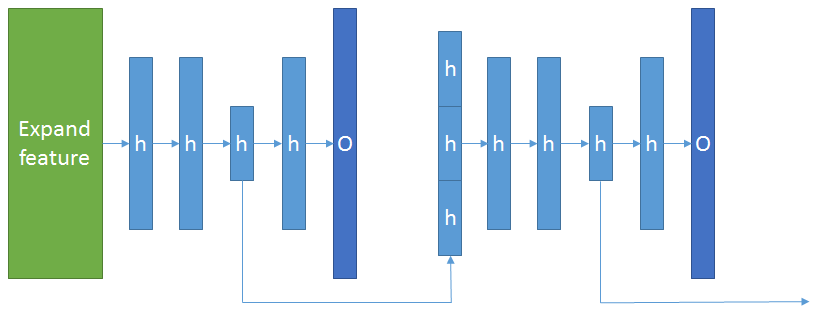
\includegraphics[width=0.9\linewidth]{tandem.png}
\end{center}

\subsection*{Keyword Boosted Language Model}
\begin{itemize}
\setlength \itemsep{0.2em}
\item A unigram language model is trained on all keywords.
\item Interpolate keyword unigram LM with default word language model to get $G_{boost}$.
\item Rescore transduced word lattices 
\end{itemize}
\begin{equation}
\hat Lat_{syl} \circ L_{syl2wrd} \circ G_{boost}
\end{equation}
}

%%%%%%%%%%%%%%%%%%%%%%%%%%%%%%%%%%%%%%%%%%%%%%%%%%%%%%%%%%%%%%%%%%%%%%%%%%%%%%
\headerbox{Experiments}{name=experiments,column=2,row=0}{
%%%%%%%%%%%%%%%%%%%%%%%%%%%%%%%%%%%%%%%%%%%%%%%%%%%%%%%%%%%%%%%%%%%%%%%%%%%%%%
\subsection*{Langauge Pack Statistics}
\begin{center}
  \captionof{table}{BABEL data used in this paper}
  \begin{tabular}{c|c|c}
    \hline
              & version     & kwlist\\
    \hline
    Assamese & IARPA-babel102b-v0.5a   & conv-eval.kwlist4 \\
    Bengali  & IARPA-babel103b-v0.4b   & conv-eval.kwlist4 \\
    Creole   & IARPA-babel201b-v0.2b   & conv-eval.kwlist4 \\
    Zulu      & IARPA-babel206b-v0.1e  & conv-eval.kwlist4 \\
    Tamil     & IARPA-babel204b-v1.1b  & conv-eval.kwlist5 \\
    \hline
  \end{tabular}
\end{center}
\vspace{-1.3em}

\subsection*{Recognition Setup}
\begin{itemize}
\setlength \itemsep{0.2em}
\item The Kaldi toolkit for the speech recognition.
\item PLP + pitch feature.
\item GMM-HMM => DNN-HMM hybrid system.
\item Position-independent phones.
\item Index based lattice search for KWS.
\end{itemize}
\vspace{-1em}

\subsection*{KWS Setup}
\begin{itemize}
\setlength \itemsep{0.2em}
\item Empirical threasholding for lattice-index-based KWS
\item Nelder Mead optimization for KWS parameter tuning
\item KST score normalization for all the methods
\end{itemize}
}

%%%%%%%%%%%%%%%%%%%%%%%%%%%%%%%%%%%%%%%%%%%%%%%%%%%%%%%%%%%%%%%%%%%%%%%%%%%%%%
\headerbox{Conclusion}{name=conclusion,column=2,below=experiments,above=bottom}{
%%%%%%%%%%%%%%%%%%%%%%%%%%%%%%%%%%%%%%%%%%%%%%%%%%%%%%%%%%%%%%%%%%%%%%%%%%%%%%
\begin{itemize}
\setlength \itemsep{0.2em}
\item Syllable transduction is helpful in spotting both IVs and OOVs in KWS. It tends to give a lower false alarm rate.
\item Combination of phone confusion, syllable search and syllable transduction can boost OOV ATWV
\end{itemize}
}

\end{poster}

\end{document}
